\documentclass[12pt,a4paper]{article}
\usepackage[utf8]{inputenc}
\usepackage[T1]{fontenc}
\usepackage{amsmath}
\usepackage{amsfonts}
\usepackage{amssymb}
\usepackage{graphicx}
\usepackage[indonesian]{babel}
\usepackage[left=2.00cm, right=2.00cm, top=2.00cm, bottom=2.00cm]{geometry}
\usepackage{float} 

\title{Tugas 9 - Pengolahan Sinyal Digital\\
		Discreet Fourier Transform (DFT)}

% remove spacing around date:
\usepackage{titling}
\predate{}
\postdate{}
\date{}

\begin{document}
	\maketitle
	\date{}
	\begin{enumerate}
		\item Hitunglah DFT dari masing-masing finite-length sequence berikut ini dengan asumsi panjang sequence-nya adalah $ N $
		\begin{enumerate}
			\item $ x(n)=\delta(n) $.
			\item $ x(n)=\delta(n-n_{0}) $, dimana $ 0<n_{0}<N $.
			\item $ x(n)=a^{n} $, $ 0\leq n\leq N-1 $.
		\end{enumerate}
	
		\item Diketahui suatu finite-length sequence, $ x(n) $, seperti yang ditampilkan pada Gambar \ref{fig:img01}. Gambarkan sequence $ x_1(n) $ dan $ x_2(n) $ yang mana \[ x_1(n) = x((n-2))_4 R_4(n) \] \[ x_2(n) = x((-n))_4 R_4(n) \] (Perlu diperhatikan bahwa $ x_1(n) $ adalah $ x(n) $ yang circular shifted 2 point)
		
		\begin{figure}[H]
			\centering
			
\includegraphics[width=0.5\linewidth]{img/img01}
			\caption{finite-length sequence $ x(n) $}
			\label{fig:img01}
		\end{figure}
		
		\item Gambar \ref{fig:img02} di bawah menunjukkan 2 finite length sequence. Gambarlah circular convolution 6 point-nya
		
		\begin{figure}[H]
			\centering
			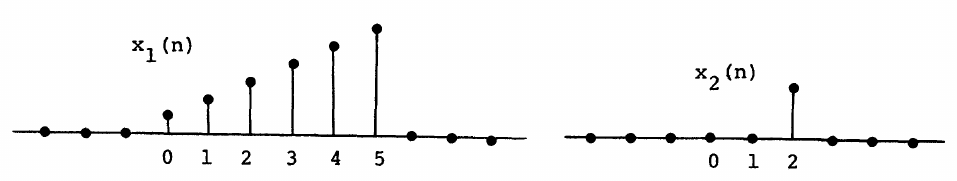
\includegraphics[width=0.7\linewidth]{img/img02}
			\caption{finite-length sequence $ x(n) $}
			\label{fig:img02}
		\end{figure}
	
	\end{enumerate}
\end{document}